% Options for packages loaded elsewhere
\PassOptionsToPackage{unicode}{hyperref}
\PassOptionsToPackage{hyphens}{url}
%
\documentclass[
  11pt,
]{article}
\usepackage{amsmath,amssymb}
\usepackage{lmodern}
\usepackage{iftex}
\ifPDFTeX
  \usepackage[T1]{fontenc}
  \usepackage[utf8]{inputenc}
  \usepackage{textcomp} % provide euro and other symbols
\else % if luatex or xetex
  \usepackage{unicode-math}
  \defaultfontfeatures{Scale=MatchLowercase}
  \defaultfontfeatures[\rmfamily]{Ligatures=TeX,Scale=1}
  \setmainfont[]{Fira Sans Condensed}
  \setmonofont[]{Fira Code}
  \setmathfont[]{Fira Sans}
\fi
% Use upquote if available, for straight quotes in verbatim environments
\IfFileExists{upquote.sty}{\usepackage{upquote}}{}
\IfFileExists{microtype.sty}{% use microtype if available
  \usepackage[]{microtype}
  \UseMicrotypeSet[protrusion]{basicmath} % disable protrusion for tt fonts
}{}
\makeatletter
\@ifundefined{KOMAClassName}{% if non-KOMA class
  \IfFileExists{parskip.sty}{%
    \usepackage{parskip}
  }{% else
    \setlength{\parindent}{0pt}
    \setlength{\parskip}{6pt plus 2pt minus 1pt}}
}{% if KOMA class
  \KOMAoptions{parskip=half}}
\makeatother
\usepackage{xcolor}
\usepackage[margin=1in]{geometry}
\usepackage{graphicx}
\makeatletter
\def\maxwidth{\ifdim\Gin@nat@width>\linewidth\linewidth\else\Gin@nat@width\fi}
\def\maxheight{\ifdim\Gin@nat@height>\textheight\textheight\else\Gin@nat@height\fi}
\makeatother
% Scale images if necessary, so that they will not overflow the page
% margins by default, and it is still possible to overwrite the defaults
% using explicit options in \includegraphics[width, height, ...]{}
\setkeys{Gin}{width=\maxwidth,height=\maxheight,keepaspectratio}
% Set default figure placement to htbp
\makeatletter
\def\fps@figure{htbp}
\makeatother
\setlength{\emergencystretch}{3em} % prevent overfull lines
\providecommand{\tightlist}{%
  \setlength{\itemsep}{0pt}\setlength{\parskip}{0pt}}
\setcounter{secnumdepth}{-\maxdimen} % remove section numbering
\usepackage{amsmath}
\usepackage{multirow, multicol, booktabs}
\ifLuaTeX
  \usepackage{selnolig}  % disable illegal ligatures
\fi
\IfFileExists{bookmark.sty}{\usepackage{bookmark}}{\usepackage{hyperref}}
\IfFileExists{xurl.sty}{\usepackage{xurl}}{} % add URL line breaks if available
\urlstyle{same} % disable monospaced font for URLs
\hypersetup{
  pdftitle={Problem Set 2},
  pdfauthor={Solutions},
  hidelinks,
  pdfcreator={LaTeX via pandoc}}

\title{Problem Set 2}
\author{Solutions}
\date{ECON 306 Fall 2022}

\begin{document}
\maketitle

\textbf{Note:} Answers may be longer than I would deem sufficient on an
exam. Some might vary slightly based on points of interest, examples, or
personal experience. These suggested answers are designed to give you
both the answer and a short explanation of why it is the answer.

\hypertarget{concepts-and-critical-thinking}{%
\section{Concepts and Critical
Thinking}\label{concepts-and-critical-thinking}}

\begin{enumerate}
\def\labelenumi{\arabic{enumi}.}
\tightlist
\item
  \textbf{Describe, in your own words, the (i) price effect, (ii) real
  income effect, and (iii) substitution effect from a price change.}
\end{enumerate}

\begin{center}\rule{0.5\linewidth}{0.5pt}\end{center}

The substitution effect is the change in consumption of a good due to a
price change; the fact that a change in price causes consumers to
substitute some of one good for another, specifically, they buy less of
the good that has become relatively more expensive, and buy more of the
good that has become relatively cheaper, and get the same utility. This
is the classic cause of a downward sloping demand curve.

The ``real'' income effect is the change in consumption of a good due to
a change in real purchasing power arising from a price change (now you
can buy more goods in total because at least one good is cheaper). This
may be positive or negative, depending on whether the good is a normal
good (positive) or an inferior good (negative).

The price effect is the overall net effect, adding the income and
substitution effects together to describe the change in consumption from
a change in that good's price.

\begin{center}\rule{0.5\linewidth}{0.5pt}\end{center}

\begin{enumerate}
\def\labelenumi{\arabic{enumi}.}
\setcounter{enumi}{1}
\tightlist
\item
  \textbf{Under what conditions can the law of demand be violated
  (however theoretical)?}
\end{enumerate}

\begin{center}\rule{0.5\linewidth}{0.5pt}\end{center}

A ``Giffen good'' violates the law of demand, that is, as price
increases (decreases), the quantity demanded for the good also increases
(decreases). The good must be (i) an inferior good (negative real income
effect) and the (ii) real income effect must be larger than the
substitution effect.

\clearpage

\begin{enumerate}
\def\labelenumi{\arabic{enumi}.}
\setcounter{enumi}{2}
\tightlist
\item
  \textbf{For each of the following pairs, which of the two goods is
  more likely to have a \emph{low} price elasticity of demand (less
  elastic) and why?}
\end{enumerate}

\begin{enumerate}
\def\labelenumi{\alph{enumi}.}
\tightlist
\item
  \textbf{Demand for tangerines vs.~demand for fruit}
\end{enumerate}

\begin{center}\rule{0.5\linewidth}{0.5pt}\end{center}

Fruit is more inelastically demanded because the overall category of
fruit has fewer good substitutes than any one item in that category.

\begin{center}\rule{0.5\linewidth}{0.5pt}\end{center}

\begin{enumerate}
\def\labelenumi{\alph{enumi}.}
\setcounter{enumi}{1}
\tightlist
\item
  \textbf{Demand for beef next month vs.~demand for beef over the next
  decade}
\end{enumerate}

\begin{center}\rule{0.5\linewidth}{0.5pt}\end{center}

More inelastic over the next month because people are usually less
flexible in their buying behavior in the short run.

\begin{center}\rule{0.5\linewidth}{0.5pt}\end{center}

\begin{enumerate}
\def\labelenumi{\alph{enumi}.}
\setcounter{enumi}{2}
\tightlist
\item
  \textbf{Demand for Exxon gasoline at the corner of 7th and Grand
  vs.~demand for gasoline in the entire city}
\end{enumerate}

\begin{center}\rule{0.5\linewidth}{0.5pt}\end{center}

Brand-named goods are more elastic than categories especially when there
are very good substitutes for Exxon gasoline available at close
distances.

\begin{center}\rule{0.5\linewidth}{0.5pt}\end{center}

\begin{enumerate}
\def\labelenumi{\alph{enumi}.}
\setcounter{enumi}{3}
\tightlist
\item
  \textbf{Demand for insulin vs.~demand for vitamins}
\end{enumerate}

\begin{center}\rule{0.5\linewidth}{0.5pt}\end{center}

Insulin is probably more of a necessity; thus, demand for insulin from
buyers is more inelastic than demand for vitamins for buyers of
vitamins.

\clearpage

\begin{enumerate}
\def\labelenumi{\arabic{enumi}.}
\setcounter{enumi}{3}
\tightlist
\item
  \textbf{Suppose that, holding prices constant, Alice has preferences
  over the number of books she purchases, illustrated in the table
  below.}
\end{enumerate}

\begin{table}
\centering
\begin{tabular}{rr}
\toprule
Income & Books\\
\midrule
5 & 5\\
10 & 6\\
15 & 20\\
20 & 25\\
25 & 26\\
\addlinespace
30 & 10\\
35 & 9\\
40 & 8\\
45 & 7\\
50 & 6\\
\bottomrule
\end{tabular}
\end{table}

\textbf{Draw a smooth approximation of Alice's Engel curve for books,
indicating the ranges over which books are inferior goods and over which
they are normal goods.}

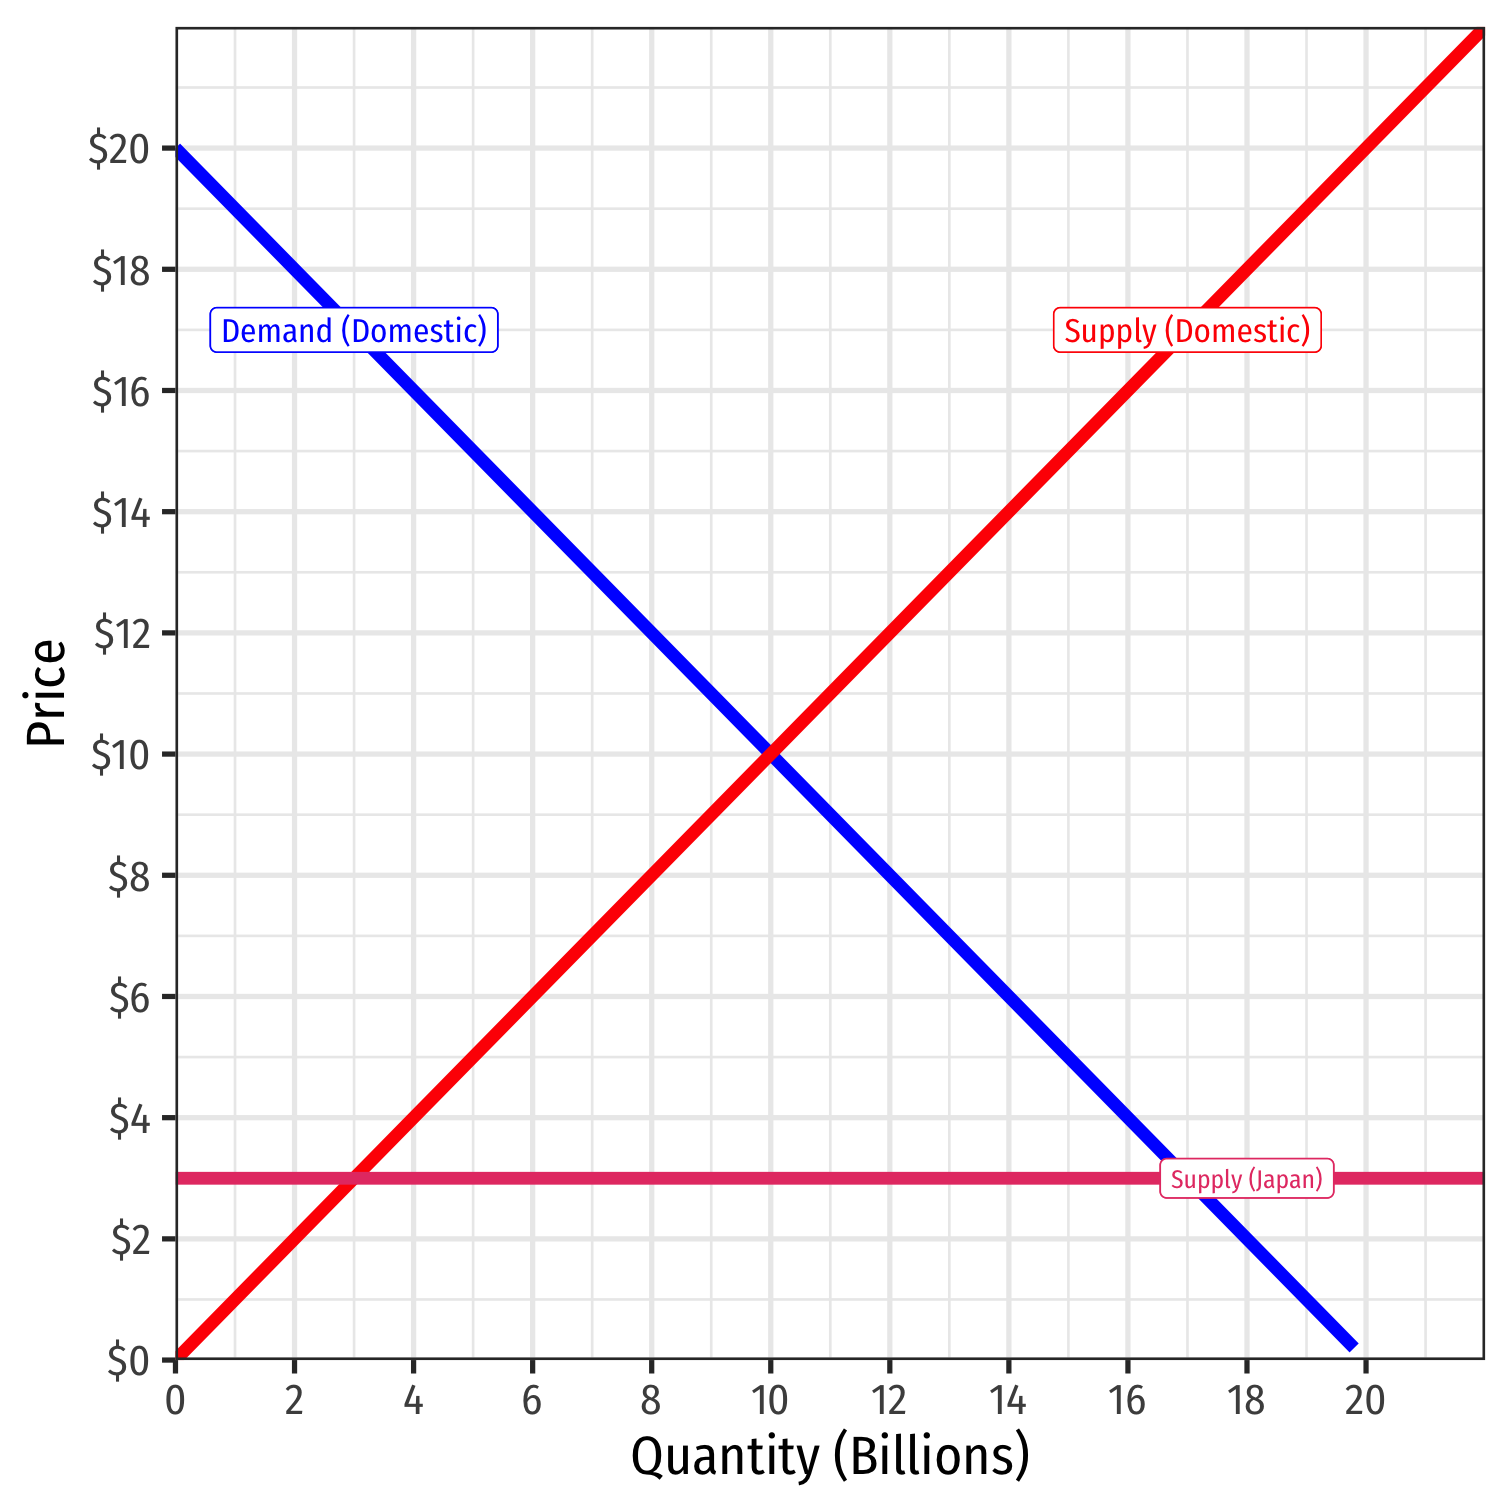
\includegraphics{02-problem-set-answers-pdf_files/figure-latex/unnamed-chunk-2-1.pdf}

Below \$20 of income, books are a normal good (the Engel curve slopes to
the upwards, so as income increases, so does consumption), but above
\$20, books become an inferior good (the Engel curve slopes to
downwards, so as income increases, so consumption decreases).

Note, you can swap the axes (Books on horizontal axis, Income on
vertical axis) like the textbook does. Either way, you should obtain the
same normal/inferior relationships at the same income ranges!

\clearpage

\hypertarget{quantitative-applications}{%
\section{Quantitative Applications}\label{quantitative-applications}}

Show all work for calculations. You may lose points, even if correct,
for missing work. Be sure to label graphs fully, if appropriate.

\begin{enumerate}
\def\labelenumi{\arabic{enumi}.}
\setcounter{enumi}{4}
\tightlist
\item
  \textbf{Steve spends his disposable income on meals at restaurants
  \((r)\) and paperback novels \((n)\). His usual restaurant meal costs
  \$25, and paperback books cost \$8. When Steve's monthly income is
  \$240, he goes out to eat 8 times and purchases 5 books. When his
  income rises to \$282, he goes out to eat 10 times and purchases 4
  books.}
\end{enumerate}

\begin{enumerate}
\def\labelenumi{\alph{enumi}.}
\tightlist
\item
  \textbf{Calculate the income elasticity for meals at restaurants
  \((r)\). Is this an inferior, necessity, or luxury good?}
\end{enumerate}

\begin{center}\rule{0.5\linewidth}{0.5pt}\end{center}

We need to examine the income elasticity of each good. Let's start with
restaurant meals:

\[\begin{aligned}
    \epsilon_{r,m}&=\cfrac{\frac{\Delta r}{r}}{\frac{\Delta m}{m}}\\
    &=\cfrac{\frac{(10-8)}{8}}{\frac{(282-240)}{240}}\\
    &=\cfrac{\frac{2}{8}}{\frac{42}{240}}\\
    &=\frac{0.25}{0.175}\\
    &\approx 1.43
    \end{aligned}\]

Since the elasticity is positive, they are normal goods. Since the
elasticity is larger than 1, they are luxury goods. For every 1\%
Steve's income increases (decreases), he buys 1.43\% more (fewer) meals.

\begin{center}\rule{0.5\linewidth}{0.5pt}\end{center}

\begin{enumerate}
\def\labelenumi{\alph{enumi}.}
\setcounter{enumi}{1}
\tightlist
\item
  \textbf{Calculate the income elasticity for paperback novels \((n)\).
  Is this an inferior, necessity, or luxury good?}
\end{enumerate}

\[\begin{aligned}
    \epsilon_{n,m}&=\cfrac{\frac{\Delta n}{n}}{\frac{\Delta m}{m}}\\
    &=\cfrac{\frac{(4-5)}{5}}{\frac{(282-240)}{240}}\\
    &=\cfrac{\frac{-1}{5}}{\frac{42}{240}}\\
    &=\frac{-0.20}{0.175}\\
    &\approx -1.14
    \end{aligned}\]

Since the elasticity is negative, they are inferior goods. For every 1\%
income increases (decreases), Steve buys 1.14\% fewer (more) novels.

\clearpage

\begin{enumerate}
\def\labelenumi{\arabic{enumi}.}
\setcounter{enumi}{5}
\tightlist
\item
  \textbf{Kendra buys eggs \((e)\), bagels \((b)\), and coffee \((c)\)
  for breakfast for the week.}
\end{enumerate}

\begin{enumerate}
\def\labelenumi{\alph{enumi}.}
\tightlist
\item
  \textbf{When eggs are \$2/carton, she buys 5 bagels. When the price of
  eggs falls to \$1/carton, she buys 4 bagels. Calculate the cross-price
  elasticity between eggs and bagels. Are they complements or
  substitutes for Kendra?}
\end{enumerate}

\begin{center}\rule{0.5\linewidth}{0.5pt}\end{center}

\[\begin{aligned}
    \epsilon_{b,p_e}&=\cfrac{\frac{\Delta b}{b}}{\frac{\Delta p_e}{p_e}}\\
    &=\cfrac{\frac{(4-5)}{5}}{\frac{(1-2)}{2}}\\
    &=\cfrac{\frac{-1}{5}}{\frac{-1}{2}}\\
    &=\frac{0.2}{0.5}\\
    &=0.4\\
    \end{aligned}\]

Since the cross-price elasticity is positive, they are substitutes. When
the price of eggs increases (decreases) by 1\%, she buys 0.4\% more
(fewer) bagels.

\begin{center}\rule{0.5\linewidth}{0.5pt}\end{center}

\begin{enumerate}
\def\labelenumi{\alph{enumi}.}
\setcounter{enumi}{1}
\tightlist
\item
  \textbf{When eggs are \$2/carton, she buys 3 cups of coffee. When the
  price of eggs falls to \$1/carton, she buys 6 cups of coffee.
  Calculate the cross-price elasticity between eggs and coffee. Are they
  complements or substitutes for Kendra?}
\end{enumerate}

\begin{center}\rule{0.5\linewidth}{0.5pt}\end{center}

\[\begin{aligned}
    \epsilon_{c,p_e}&=\cfrac{\frac{\Delta c}{c}}{\frac{\Delta p_e}{p_e}}\\
    &=\cfrac{\frac{(6-3)}{3}}{\frac{(1-2)}{2}}\\
    &=\cfrac{\frac{3}{3}}{\frac{-1}{2}}\\
    &=\frac{1}{-0.5}\\
    &=-2\\
    \end{aligned}\]

Since the cross-price elasticity is negative, they are complements. When
the price of eggs increases (decreases) by 1\%, she buys 2\% fewer
(more) cups of coffee.

\clearpage

7 \textbf{Sketch a graph showing an \emph{increase} in the price of a
good (on the horizontal axis, e.g.~\(x\) if you want). Indicate the
(real) income effect, substitution effect, and price effect on the
graph. Labelling points and describing each effect as a movement between
specific points is sufficient.}

\begin{center}\rule{0.5\linewidth}{0.5pt}\end{center}

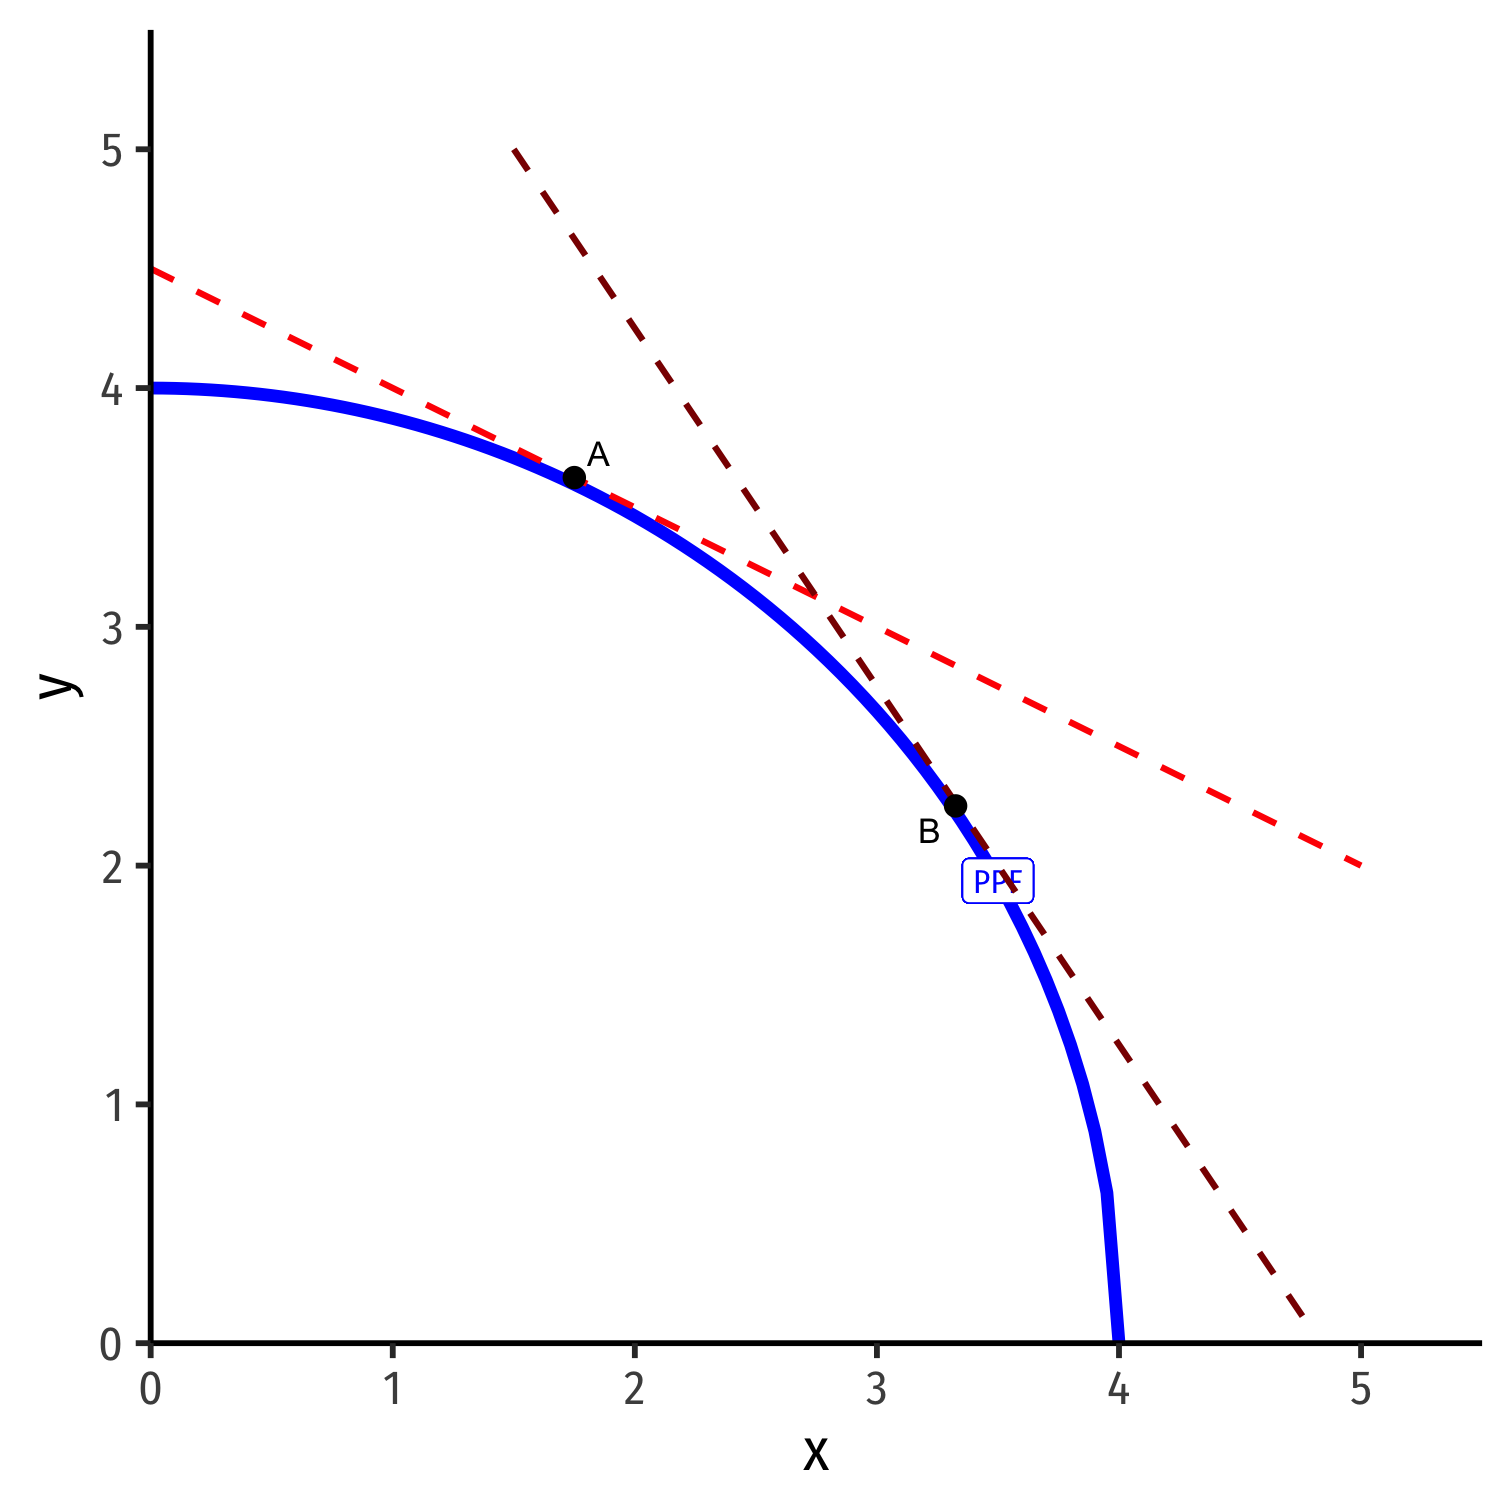
\includegraphics{../slides/1.6-slides_files/figure-html/unnamed-chunk-12-1.png}

We begin with an original optimum at point \(A\). Then the price of
\(x\) rises from \(1.00\) to \(2.00\):

The \textbf{substitution effect} (orange) is where we shift the new
budget line \(BC_2\) (reflecting the new relative prices of \(x\) and
\(y\)) outwards until it is tangent to the original indifference curve
\((u_1)\) at a different point, in this case, point B. This tells us,
under the new prices, how much \(x\) and \(y\) the person would want to
consume to enjoy the same level of utility (she substitutes more \(y\)
for less \(x\)).

The \textbf{real income effect} (green) is where the change in price
allows the consumer to purchase more goods than before, where she must
move to a lower indifference curve \((u_0)\) at point C. From point B,
she consumes less \(x\) and less \(y\).

Thus, the \textbf{total price effect} (purple), moving from A to C, when
the price of \(x\) rises, is for her to buy less \(x\) (and no change in
\(y)\).

\clearpage

\begin{enumerate}
\def\labelenumi{\arabic{enumi}.}
\setcounter{enumi}{7}
\tightlist
\item
  \textbf{8. The demand for gym memberships is given by} \[q_D=500-5p\]
\end{enumerate}

\begin{enumerate}
\def\labelenumi{\alph{enumi}.}
\tightlist
\item
  \textbf{Write the inverse demand function.}
\end{enumerate}

\begin{center}\rule{0.5\linewidth}{0.5pt}\end{center}

\[\begin{aligned}
    q_D&=500-5p\\
    q_D-500&=-5p\\
    100-\frac{1}{5}&=p\\
    \end{aligned}\]

\begin{center}\rule{0.5\linewidth}{0.5pt}\end{center}

\begin{enumerate}
\def\labelenumi{\alph{enumi}.}
\setcounter{enumi}{1}
\tightlist
\item
  \textbf{Calculate the price elasticity of demand at a price of \$80.
  Is this relatively elastic or relatively inelastic?}
\end{enumerate}

\begin{center}\rule{0.5\linewidth}{0.5pt}\end{center}

First, we need to find the quantity demanded when price is \$80:

\[\begin{aligned}
    q_D&=500-5p\\
    q_D&=500-5(80)\\
    q_D&=500-400\\
    q_D&=100\\
    \end{aligned}\]

We found the slope from the inverse demand curve, \(-\frac{1}{5}\).

Now that we have the price (\$80), quantity demanded (100) and the slope
\((-\frac{1}{5})\), we can plug these into the formula for point
elasticity of demand:

\[\begin{aligned}
    \epsilon_D &= \frac{1}{slope} \times \frac{p}{q_D}\\
    \epsilon_D &= \cfrac{1}{\left(-\frac{1}{5}\right)} \times \frac{80}{100}\\ 
    \epsilon_D &= -5 \times 0.8 \\
    \epsilon_D &= -4\\ 
    \end{aligned}\]

Since \(|\epsilon_D| >1\), this is relatively elastic. For every 1\%
price increases (decreases), quantity demanded decreases (increases) by
4\%.

\begin{center}\rule{0.5\linewidth}{0.5pt}\end{center}

\begin{enumerate}
\def\labelenumi{\alph{enumi}.}
\setcounter{enumi}{2}
\tightlist
\item
  \textbf{What is the total revenue at a price of \$80?}
\end{enumerate}

\begin{center}\rule{0.5\linewidth}{0.5pt}\end{center}

\[\begin{aligned}
    R&=pq   \\
    R&=(\$80)(100)\\
    R&=\$8,000  \\
    \end{aligned}\]

\begin{center}\rule{0.5\linewidth}{0.5pt}\end{center}

\begin{enumerate}
\def\labelenumi{\alph{enumi}.}
\setcounter{enumi}{3}
\tightlist
\item
  \textbf{Calculate the price elasticity of demand at a price of \$10.
  Is this relatively elastic or relatively inelastic?}
\end{enumerate}

\begin{center}\rule{0.5\linewidth}{0.5pt}\end{center}

Now we need the quantity demanded when price is \$10:

\[\begin{aligned}
    q_D&=500-5p\\
    q_D&=500-5(10)\\
    q_D&=500-50\\
    q_D&=450    \\
    \end{aligned}\]

We have the price (\$10), quantity demanded (450) and the slope
\((-\frac{1}{5})\), we can plug these into the formula for point
elasticity of demand:

\[\begin{aligned}
    \epsilon_D &= \frac{1}{slope} \times \frac{p}{q_D}\\    
    \epsilon_D &= \cfrac{1}{-\frac{1}{5}} \times \frac{10}{450} \\
    \epsilon_D &= -5 \times 0.02\\
    \epsilon_D &\approx -0.11   \\
    \end{aligned}\]

Since \(|\epsilon_D| < 1\), this is relatively inelastic. For every 1\%
price increases (decreases), quantity demanded decreases (increases) by
0.11\%.

\begin{center}\rule{0.5\linewidth}{0.5pt}\end{center}

\begin{enumerate}
\def\labelenumi{\alph{enumi}.}
\setcounter{enumi}{4}
\tightlist
\item
  \textbf{What is the total revenue at \$10?}
\end{enumerate}

\begin{center}\rule{0.5\linewidth}{0.5pt}\end{center}

\[\begin{aligned}
    R&=pq   \\
    R&=(\$10)(450)\\
    R&=\$4,500  \\
    \end{aligned}\]

\begin{center}\rule{0.5\linewidth}{0.5pt}\end{center}

\begin{enumerate}
\def\labelenumi{\alph{enumi}.}
\setcounter{enumi}{5}
\tightlist
\item
  \textbf{At what price is demand unit elastic, i.e.~\(\epsilon_D=-1\)?}
\end{enumerate}

\begin{center}\rule{0.5\linewidth}{0.5pt}\end{center}

We can solve for the price by using the elasticity of demand formula,
setting it equal to -1, and plugging the righthand side of the demand
equation in for \(q_D\), since \(q_D=500-5p\).

\[\begin{aligned}
    \epsilon_D &= \frac{1}{slope} \times \frac{p}{q_D}\\ 
    -1 &= -5 \times \frac{p}{(500-5p)}\\
    -1(500-5p)&=-5p\\   
    -500+5p&=-5p\\
    -500&=-10p\\
    50&=p\\
    \end{aligned}\]

\begin{center}\rule{0.5\linewidth}{0.5pt}\end{center}

\begin{enumerate}
\def\labelenumi{\alph{enumi}.}
\setcounter{enumi}{6}
\tightlist
\item
  \textbf{What is the total revenue at the price you find in part (f)?}
\end{enumerate}

\begin{center}\rule{0.5\linewidth}{0.5pt}\end{center}

We have the price, but we need to find the quantity demanded at \$50.

\[\begin{aligned}
    q_D &= 500-5p\\
    q_D&=500-5(50)\\
    q_D&=500-250\\
    q_D& = 250  \\
    \end{aligned}\]

Now we can calculate the total revenue.

\[\begin{aligned}
    R&=pq   \\
    R&=(\$50)(250)\\
    R&=\$12,500 \\
    \end{aligned}\]

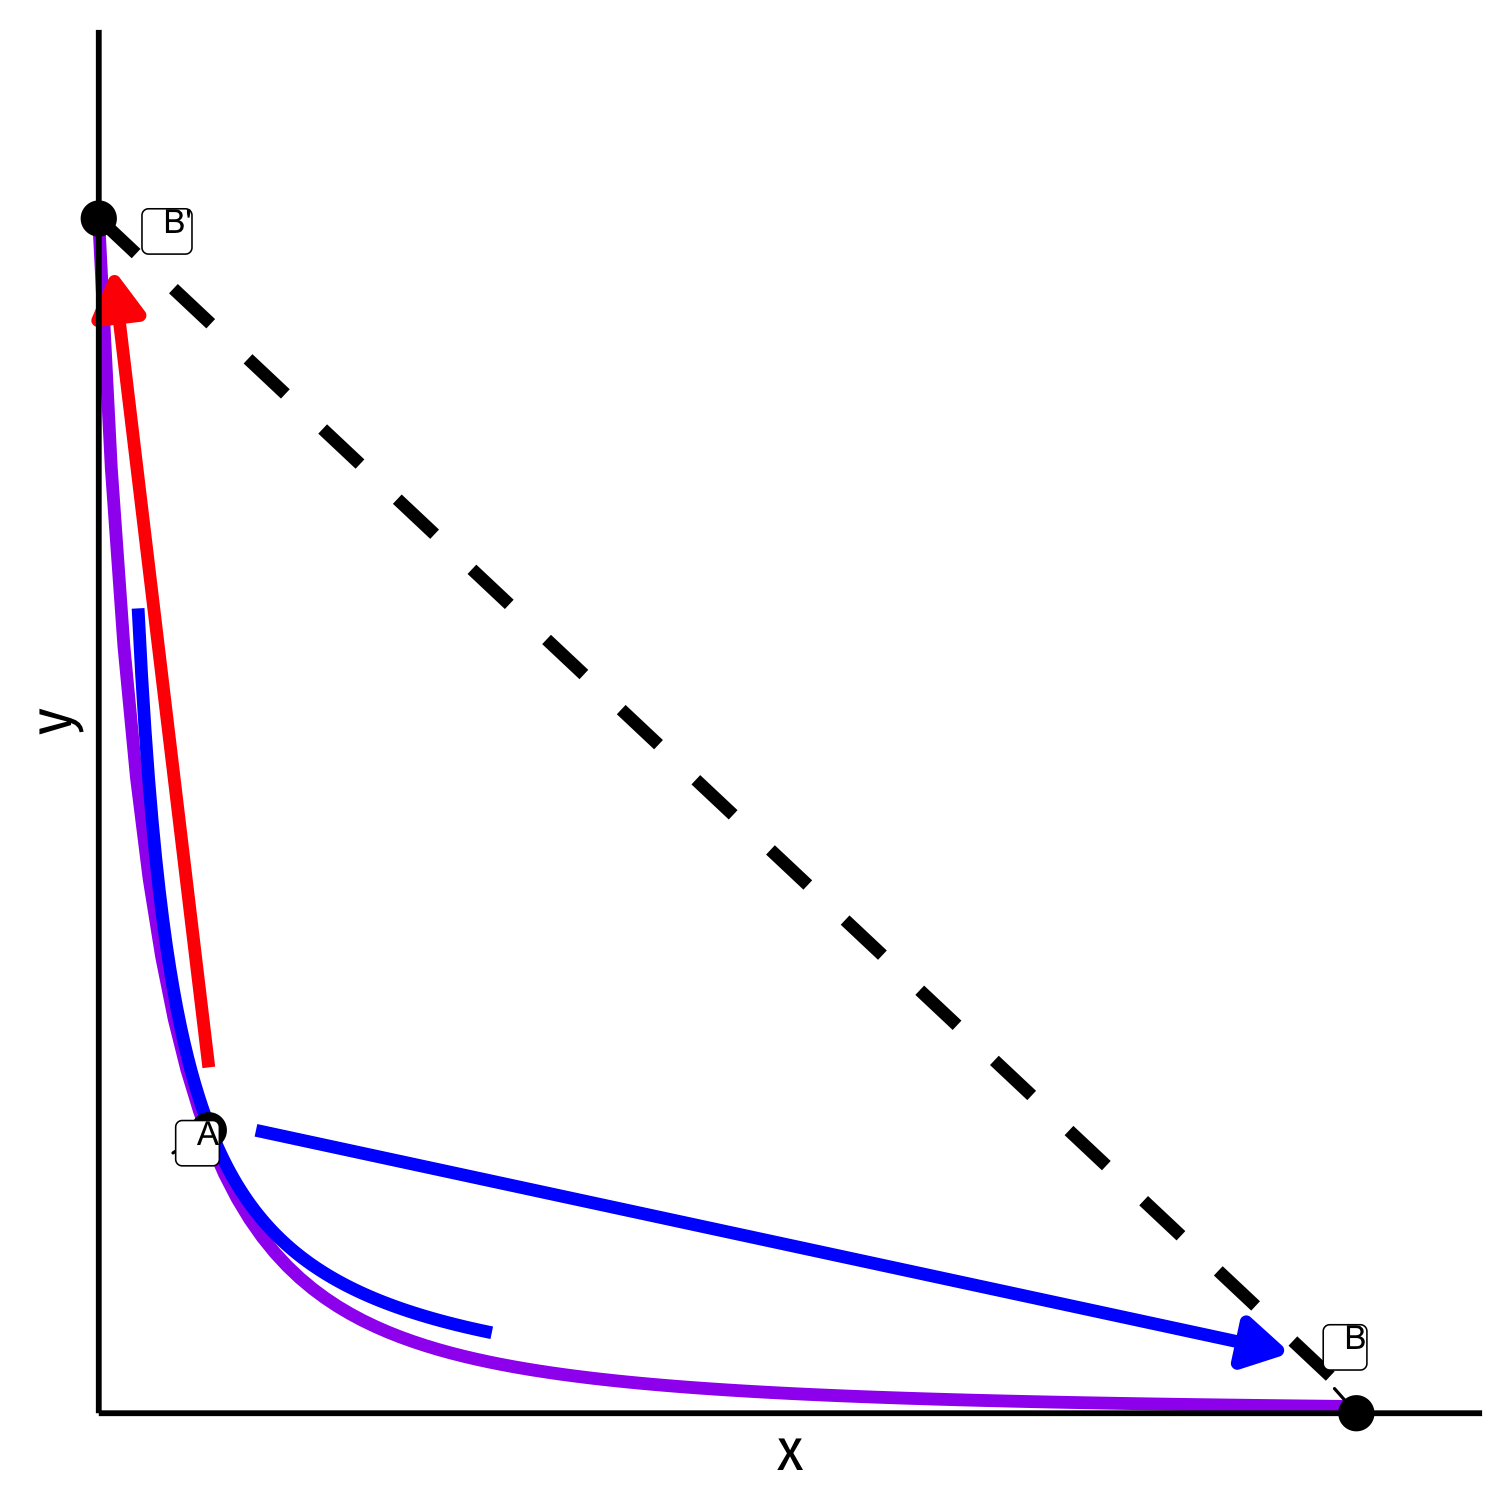
\includegraphics{02-problem-set-answers-pdf_files/figure-latex/unnamed-chunk-3-1.pdf}

\end{document}
